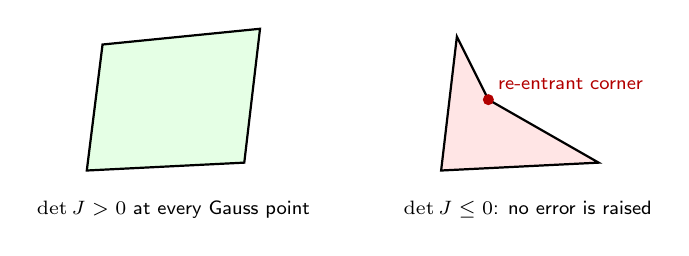
\begin{tikzpicture}[font=\sffamily\scriptsize]
\draw[fill=green!10,thick] (0,0) -- (2,0.1) -- (2.2,1.8) -- (0.2,1.6) -- cycle;
\node at (1.1,-0.5) {$\det\bm J>0$ at every Gauss point};
\draw[fill=red!10,thick] (4.5,0) -- (6.5,0.1) -- (5.1,0.9) -- (4.7,1.7) -- cycle;
\fill[red!70!black] (5.1,0.9) circle (2pt) node[above right] {re-entrant corner};
\node at (5.6,-0.5) {$\det\bm J\le0$: no error is raised};
\end{tikzpicture}
